% CIPAT Project Report Format
% Font: Times New Roman / Calibri, Size: 12, Line Spacing: 1.5
\documentclass[12pt,a4paper]{article}

% Page layout
\usepackage[margin=1in]{geometry}
\usepackage{parskip}
\usepackage{setspace}
\onehalfspacing
\setlength{\parskip}{0.7em plus 0.25em minus 0.1em}

% Font: Times New Roman
\usepackage{mathptmx}
\usepackage[T1]{fontenc}

% Justified paragraphs
\usepackage{ragged2e}
\justifying
% Reduce overfull/underfull boxes
\sloppy
\setlength{\emergencystretch}{1.5em}

% Uniform spacing between blocks (diagrams, sections, explanations)
\newcommand{\blocksep}{\medskip}

% Table of contents and sections
\usepackage{tocloft}
\usepackage{titlesec}
\usepackage{enumitem}
% More space in lists and after headings
\setlist{itemsep=0.35em, parsep=0.2em, topsep=0.4em}
\titlespacing*{\section}{0pt}{1.2em}{0.6em}
\titlespacing*{\subsection}{0pt}{1em}{0.5em}
\titlespacing*{\subsubsection}{0pt}{0.8em}{0.4em}
\titleformat{\section}{\fontsize{16pt}{19.2pt}\selectfont\bfseries}{\thesection.}{0.5em}{}
\titleformat{\subsection}{\fontsize{14pt}{16.8pt}\selectfont\bfseries}{\thesubsection}{0.5em}{}
\titleformat{\subsubsection}{\fontsize{12pt}{18pt}\selectfont\bfseries}{\thesubsubsection}{0.5em}{}
\setcounter{secnumdepth}{3}
\setcounter{tocdepth}{2}
\usepackage{graphicx}
\usepackage{adjustbox}
\usepackage{booktabs}
\usepackage{longtable}
\usepackage{array}
\usepackage{listings}
\usepackage{xcolor}
\usepackage{url}
\usepackage{float}

% Hyperref for references
\usepackage{hyperref}
\hypersetup{colorlinks=true, linkcolor=black, urlcolor=blue}

% Header and footer
\usepackage{lastpage}
\usepackage{fancyhdr}
\setlength{\headheight}{15pt}
\pagestyle{fancy}
\fancyhf{}
\fancyhead[L]{\subjectname}
\fancyhead[R]{Project: \projecttitle}
\fancyfoot[C]{\thepage\ of \pageref{LastPage}}
\renewcommand{\headrulewidth}{0pt}
\renewcommand{\footrulewidth}{0pt}
\fancypagestyle{plain}{\fancyhf{}\fancyfoot[C]{\thepage\ of \pageref{LastPage}}\renewcommand{\headrulewidth}{0pt}}

% ========== SET YOUR DETAILS HERE ==========
\newcommand{\projecttitle}{Secure Credential Sharing System}
\newcommand{\subjectname}{Software Engineering}
\newcommand{\facultyname}{Prof Priyanka Afini}
\newcommand{\submissiondate}{09/03/2026}
% Team Members: (Name, Enrollment No.)
\newcommand{\teammemberone}{Patil Devendra Vinod -- 230090116054}
\newcommand{\teammembertwo}{Vala Shakti Pratapbhai -- 230090116065}
\newcommand{\teammemberthree}{Patil Bhavesh Shashikant -- 240093116002}
% ==========================================

\title{\fontsize{16pt}{19.2pt}\selectfont \projecttitle}
\author{\subjectname\\[0.5em]
  Team Members: \teammemberone, \teammembertwo, \teammemberthree\\
  Faculty: \facultyname\\
  Date: \submissiondate}
\date{}

\begin{document}

% --- Cover Page ---
\begin{titlepage}
  \centering
  \vspace*{2cm}
  {\fontsize{20pt}{24pt}\selectfont \textbf{\projecttitle}\par}
  \vspace{1.5cm}
  {\fontsize{14pt}{16.8pt}\selectfont \subjectname\par}
  \vspace{2cm}
  {\fontsize{12pt}{18pt}\selectfont
    \textbf{Team Members}\par
    \teammemberone\par
    \teammembertwo\par
    \teammemberthree\par
  }
  \vspace{1.5cm}
  {\fontsize{12pt}{18pt}\selectfont
    \textbf{Faculty Name:}\ \facultyname\par
    \textbf{Submission Date:}\ \submissiondate\par
  }
  \vfill
\end{titlepage}

% Reset page style for rest of document
\pagestyle{fancy}
\pagenumbering{roman}
\setcounter{page}{2}

% --- Table of Contents ---
\tableofcontents
\newpage

% --- Main Content ---
\pagenumbering{arabic}
\setcounter{page}{1}

\fontsize{12pt}{18pt}\selectfont

% ==================== 1. Introduction ====================
\section{Introduction}

\subsection{Problem Understanding}

In today's digital landscape, organizations and individuals frequently need to share sensitive information such as API keys, passwords, configuration files, and temporary credentials with team members, external partners, and automated systems. Current methods of sharing this information---email, instant messaging, plain text files, or password-protected documents---are inherently insecure and pose significant security risks.

\textbf{Key Problems Identified:}
\begin{enumerate}[leftmargin=*]
  \item \textbf{Security Vulnerabilities:} Traditional communication channels are often unencrypted or logged, leaving sensitive data exposed to interception, unauthorized access, and data breaches.
  \item \textbf{Lack of Control:} Once credentials are shared via traditional methods, the sender loses control over who can access them, how many times they're viewed, and for how long they remain accessible.
  \item \textbf{No Audit Trail:} Most existing solutions lack comprehensive logging, making it impossible to track who accessed what information and when---critical for compliance and security investigations.
  \item \textbf{Poor User Experience:} Security tools often sacrifice usability for security, leading to workarounds that compromise security.
  \item \textbf{Scalability Issues:} As organizations grow, managing access permissions across multiple teams, projects, and external stakeholders becomes increasingly complex.
  \item \textbf{Compliance Requirements:} Organizations must adhere to various security standards (SOC 2, HIPAA, GDPR, PCI-DSS) that require specific security controls for sensitive data handling.
\end{enumerate}

\subsubsection{Problem Statement}

\textbf{Develop a secure, user-friendly credential sharing platform that enables organizations and individuals to share sensitive information with granular access controls, comprehensive audit logging, and end-to-end encryption while maintaining a seamless user experience.}

\textbf{Project Scope:}\\
The Secure Credential Sharing System (Secret Drop) will provide: secure storage and sharing of secrets with AES-256 encryption; time-limited and view-limited access to shared secrets; organizational hierarchy with role-based access control (RBAC); team-based collaboration within organizations; comprehensive audit logging for compliance; multiple authentication methods (email/password, SSO, 2FA); API access for automation and CI/CD integration; multi-tier subscription plans for different organizational needs.

\subsubsection{Existing System (if any)}

\textbf{Current Methods in Use:}
\begin{itemize}[leftmargin=*]
  \item \textbf{Email and Instant Messaging:} Ubiquitous and easy to use, but messages stored on servers, logs retained indefinitely, no access control, no expiration mechanism, vulnerable to forwarding.
  \item \textbf{Password-Protected Documents:} Can contain multiple secrets, but passwords shared insecurely, no audit trail, difficult to revoke access.
  \item \textbf{Commercial Password Managers (1Password, LastPass, Bitwarden):} Strong encryption for personal use, but expensive for temporary sharing, requires recipient account, complex permission management.
  \item \textbf{Self-Hosted Solutions (HashiCorp Vault, AWS Secrets Manager):} Enterprise-grade security, but high operational overhead, expensive, complex setup.
  \item \textbf{Paste-Based Solutions (Pastebin, PrivateBin):} Simple and free, but limited security features, no organizational features, weak audit capabilities.
\end{itemize}

\begin{table}[H]
  \centering
  \small
  \caption{Gaps in Existing Solutions}
  \begin{tabular}{@{}lccccc@{}}
    \toprule
    \textbf{Feature Gap}          & \textbf{Email/IM} & \textbf{Password Mgrs} & \textbf{Vault} & \textbf{Paste Tools} \\
    \midrule
    End-to-End Encryption         & No                & Yes                    & Yes            & Partial              \\
    \hline
    Time-Based Expiration         & No                & No                     & Limited        & Yes                  \\
    \hline
    View Count Limits             & No                & No                     & No             & Partial              \\
    \hline
    Burn-on-Read                  & No                & No                     & No             & Partial              \\
    \hline
    Comprehensive Audit Logs      & No                & Limited                & Yes            & No                   \\
    \hline
    Organizational Features       & No                & Limited                & Yes            & No                   \\
    \hline
    Team-Based Access Control     & No                & Limited                & Yes            & No                   \\
    \hline
    One-Time Sharing (No Account) & Yes               & No                     & No             & Yes                  \\
    \hline
    API Access                    & No                & Limited                & Yes            & No                   \\
    \hline
    Affordable for SMBs           & Yes               & No                     & No             & Yes                  \\
    \bottomrule
  \end{tabular}
\end{table}

\subsubsection{Proposed System}

\textbf{Secret Drop} is a web-based secure credential sharing platform designed to bridge the gap between security and usability.

\textbf{Core Value Proposition:}
\begin{enumerate}[leftmargin=*]
  \item \textbf{Security-First Architecture:} Client-side encryption using AES-256-GCM; dual encryption modes (server-managed and password-derived keys); zero-knowledge architecture; all secrets encrypted at rest and in transit.
  \item \textbf{Granular Access Controls:} Time-based expiration (1h, 1d, 7d, 30d, never); view count limits (1, 2, 3, 5, 10, unlimited); burn-on-read; optional password protection on share links; IP allowlisting.
  \item \textbf{Organizational Features:} Multi-tenant architecture; team-based hierarchy; role-based access control (Owner, Admin, Member); centralized billing and management.
  \item \textbf{Comprehensive Audit Trail:} All access logged with IP and user agent; view/edit/delete/share actions tracked; exportable audit logs for compliance.
  \item \textbf{Flexible Authentication:} Email/password with PBKDF2 (100,000 iterations); social login (Google, GitHub); organization SSO (SAML/OIDC); TOTP 2FA; API tokens.
  \item \textbf{Developer-Friendly:} RESTful API; SDK for major languages; CI/CD integration examples; webhook notifications.
\end{enumerate}

\textbf{Technology Stack:} Frontend: TanStack Start (React 19), TanStack Router, Tailwind CSS 4, Shadcn UI. Backend: tRPC, Better Auth, Node.js. Database: PostgreSQL with Drizzle ORM. Hosting: Netlify with edge functions. Encryption: Web Crypto API, @noble/ciphers. Payments: Stripe (via Dodo Payments).

% ==================== 2. Requirement Analysis ====================
\section{Requirement Analysis (SRS Section)}

\subsection{Overall Description}

\subsubsection{Product Perspective}
Secret Drop follows the JAMstack architecture: Client Layer (React 19 SPA, TanStack Router, Tailwind CSS); API \& Auth Layer (tRPC endpoints, Better Auth, validation); Data Layer (PostgreSQL, Drizzle ORM, Encryption Service, Audit Logger). External interfaces: web browser, RESTful API, OAuth providers, Stripe, email service.

\subsubsection{Product Functions}
\begin{table}[H]
  \centering
  \small
  \caption{Product Functions Summary}
  \begin{tabular}{@{}p{3.5cm}p{9cm}@{}}
    \toprule
    \textbf{Function}       & \textbf{Description}                                          \\
    \midrule
    Authentication          & User registration, login, logout, password recovery, SSO, 2FA \\
    \hline
    Secret Management       & Create, read, update, delete, list secrets with encryption    \\
    \hline
    Secret Sharing          & Generate shareable links with expiration and view limits      \\
    \hline
    Organization Management & Create/manage organizations, invite members, assign roles     \\
    \hline
    Team Management         & Create teams, manage team membership                          \\
    \hline
    Access Control          & Role-based permissions, IP allowlisting, team-based access    \\
    \hline
    Audit \& Compliance     & View access logs, export reports, track secret lifecycle      \\
    \hline
    Developer API           & API token management, programmatic secret access              \\
    \hline
    Billing                 & Subscription management, payment processing, plan upgrades    \\
    \bottomrule
  \end{tabular}
\end{table}

\subsubsection{User Classes and Characteristics}
\begin{table}[H]
  \centering
  \small
  \caption{User Classes}
  \begin{tabular}{@{}p{2.8cm}p{3cm}p{4cm}p{2.2cm}@{}}
    \toprule
    \textbf{User Class} & \textbf{Description}        & \textbf{Key Needs}                         & \textbf{Proficiency} \\
    \midrule
    Individual Users    & Freelancers, developers     & Quick sharing, minimal setup, free tier    & Medium-High          \\
    \hline
    Team Members        & Employees in orgs           & Collaborative sharing, team secrets, audit & Medium               \\
    \hline
    Org Admins          & Owners/IT admins            & User mgmt, SSO, compliance, billing        & High                 \\
    \hline
    External Recipients & Non-users receiving secrets & Easy access, no account required           & Low-Medium           \\
    \hline
    Developers/CI-CD    & Automated systems           & Reliable API, webhooks                     & High                 \\
    \hline
    Compliance Officers & Auditors                    & Audit trails, export                       & Medium               \\
    \bottomrule
  \end{tabular}
\end{table}

\subsubsection{Assumptions \& Constraints}

\textbf{Assumptions:}
\begin{itemize}[leftmargin=*, itemsep=0.1em]
  \item Users have modern web browsers with JavaScript enabled
  \item Users have internet connectivity for web and API access
  \item Organization administrators have basic understanding of security practices
  \item Email delivery is reliable for user notifications
  \item PostgreSQL database can handle projected load with proper indexing
  \item Netlify edge functions can handle API request volume
  \item Stripe API remains available for payment processing
\end{itemize}

\textbf{Constraints:}
\begin{enumerate}[leftmargin=*, itemsep=0.2em]
  \item \textbf{Technical:} Approved stack (TanStack, tRPC, Drizzle ORM); Netlify compatibility; schema changes via migrations; client-side encryption limited to browser Web Crypto API.
  \item \textbf{Security:} AES-256 at rest; HTTPS for all API communication; SOC 2/GDPR/PCI-DSS compliance; no plaintext secrets in server logs; master key via environment variables.
  \item \textbf{Business:} Free tier 10 secrets per organization; Pro tier 100 secrets; max secret size 1\,MB; share link max 30 days; API rate 100 req/min (free tier).
  \item \textbf{Regulatory:} GDPR (right to deletion, data export); CCPA for California; audit logs 90 days minimum, 7 years maximum retention.
  \item \textbf{Performance:} API p95 $<$ 200\,ms; page load $<$ 2\,s; 10,000 concurrent users; 99.9\% uptime SLA for paid tiers.
\end{enumerate}

\subsection{Functional Requirements}

\subsubsection{Authentication}
\begin{itemize}[leftmargin=*, itemsep=0.1em]
  \item FR-AUTH-1: Allow user registration with email and password
  \item FR-AUTH-2: Login via email/password or OAuth (Google, GitHub)
  \item FR-AUTH-3: Password reset via email
  \item FR-AUTH-4: Minimum 8-character password
  \item FR-AUTH-5: PBKDF2 with 100,000 iterations
  \item FR-AUTH-6: TOTP 2FA
  \item FR-AUTH-7: Backup codes for 2FA recovery
  \item FR-AUTH-8: Session management with configurable expiration
  \item FR-AUTH-9: Organization SSO (SAML/OIDC)
  \item FR-AUTH-10: RBAC (Owner, Admin, Member)
  \item FR-AUTH-11: API token creation, display prefix, track usage, revocation
\end{itemize}

\subsubsection{Secret Management}
\begin{itemize}[leftmargin=*, itemsep=0.1em]
  \item FR-SCRT-1: Create secrets in organization
  \item FR-SCRT-2: AES-256-GCM encryption
  \item FR-SCRT-3: Server-managed and password-derived encryption modes
  \item FR-SCRT-4: Secret name up to 255 characters
  \item FR-SCRT-5: Secret content up to 1 MB
  \item FR-SCRT-6: Assign secrets to teams
  \item FR-SCRT-7: View, edit, delete secrets
  \item FR-SCRT-8: Expiration (1h, 1d, 7d, 30d, never)
  \item FR-SCRT-9: View limits (1, 2, 3, 5, 10, unlimited)
  \item FR-SCRT-10: Burn-on-read mode
  \item FR-SCRT-11: Increment view count; prevent expired/max-view access
  \item FR-SCRT-12: List, filter, search secrets
\end{itemize}

\subsubsection{Secret Sharing}
\begin{itemize}[leftmargin=*, itemsep=0.1em]
  \item FR-SHR-1: Generate shareable links
  \item FR-SHR-2: 64-character unique tokens
  \item FR-SHR-3: Optional password protection on share links
  \item FR-SHR-4: Expiration and max view count per share link
  \item FR-SHR-5: Anonymous access via valid share links
  \item FR-SHR-6: Password validation for protected links
  \item FR-SHR-7: Track view count; prevent expired/max-view access
  \item FR-SHR-8: Revoke share links; list active shares
\end{itemize}

\subsubsection{Organization \& Team}
\begin{itemize}[leftmargin=*, itemsep=0.1em]
  \item FR-ORG-1: Create orgs; invite members; assign roles; remove/leave; multi-org membership; secret limits by tier
  \item FR-TEAM-1: Create teams; add/remove members; team secret access; delete teams
\end{itemize}

\subsubsection{Audit, Security, Billing}
\begin{itemize}[leftmargin=*, itemsep=0.1em]
  \item FR-AUDIT-1: Log view/edit/delete/share; IP and user agent; filter, export; 90-day retention
  \item FR-SEC-1: IP allowlist; AES-256; unique IV; key rotation; encrypted SSO secrets
  \item FR-BILL-1: Free/Pro/Business tiers; 10/100/unlimited secrets; Stripe; upgrade/downgrade; invoices
\end{itemize}

\subsection{Non-Functional Requirements}

\subsubsection{Performance}
\begin{itemize}[leftmargin=*, itemsep=0.1em]
  \item NFR-PERF-1: API response time p95 $<$ 200ms, p99 $<$ 500ms
  \item NFR-PERF-2: Page load $<$ 2 seconds, time to interactive $<$ 3 seconds
  \item NFR-PERF-3: Support 10,000 concurrent users
  \item NFR-PERF-4: Database query p95 $<$ 100ms for indexed queries
  \item NFR-PERF-5: Encryption/decryption $<$ 50ms for 1MB payload
\end{itemize}

\subsubsection{Security}
\begin{itemize}[leftmargin=*, itemsep=0.1em]
  \item NFR-SEC-1: TLS 1.3 for all data in transit
  \item NFR-SEC-2: AES-256-GCM at rest
  \item NFR-SEC-3: PBKDF2 with 100,000 iterations for passwords
  \item NFR-SEC-4: Cryptographically secure tokens
  \item NFR-SEC-5: Protection against SQL injection, XSS, CSRF
  \item NFR-SEC-6: Rate limiting; brute-force protection (5 attempts/15 min)
  \item NFR-SEC-7: No secret content in logs
  \item NFR-SEC-8: CSP, HSTS; SOC 2, GDPR compliant
\end{itemize}

\subsubsection{Usability}
\begin{itemize}[leftmargin=*, itemsep=0.1em]
  \item NFR-USE-1: WCAG 2.1 AA accessibility
  \item NFR-USE-2: Responsive (320px--1024px+)
  \item NFR-USE-3: Critical flows completable in $<$ 5 clicks
  \item NFR-USE-4: Inline validation; clear error messages
  \item NFR-USE-5: Keyboard navigation; onboarding
\end{itemize}

\subsubsection{Reliability}
\begin{itemize}[leftmargin=*, itemsep=0.1em]
  \item NFR-REL-1: 99\% uptime (free tier), 99.9\% (paid tiers)
  \item NFR-REL-2: 11-nines data durability
  \item NFR-REL-3: MTTR $<$ 1 hour
  \item NFR-REL-4: Daily backups; 30-day point-in-time recovery
  \item NFR-REL-5: DR RTO $<$ 4h, RPO $<$ 1h
\end{itemize}

\subsubsection{Maintainability}
\begin{itemize}[leftmargin=*, itemsep=0.1em]
  \item NFR-MAIN-1: Style guidelines; 70\% min test coverage (90\% critical paths)
  \item NFR-MAIN-2: Lint before merge; API versioning
  \item NFR-MAIN-3: Reversible migrations; health checks
  \item NFR-MAIN-4: Structured logging; documentation for all endpoints
\end{itemize}

% ==================== 3. SDLC Model Selection ====================
\section{SDLC Model Selection}

\subsection{Selected SDLC Model}

\textbf{Agile Methodology with Scrum Framework}

The Secret Drop project uses Agile development with Scrum, organized in 2-week sprints: Sprint Planning (2h); Daily Standups (15 min); Sprint Review (1h); Sprint Retrospective (30 min); Backlog Refinement (1h/week).

\subsection{Justification}

\textbf{Why Agile?} Rapidly evolving security threats need quick incorporation of patches; user feedback drives UX; market uncertainty allows feature prioritization; modern stack (TanStack, React, Drizzle) requires agile adaptation; small teams optimize with agile ceremonies.

\textbf{Why Scrum?} Time-boxed 2-week sprints balance velocity and stability; clear roles (Product Owner, Scrum Master, Dev Team); artifacts (Product Backlog, Sprint Backlog, Increment). Adaptations: CI/CD via GitHub Actions; auto-deploy to Netlify; security backlog highest priority; SOC 2/GDPR in Definition of Done.

\begin{table}[H]
  \centering
  \small
  \caption{SDLC Model Comparison}
  \begin{tabular}{@{}p{2cm}p{3cm}p{3cm}p{2.5cm}@{}}
    \toprule
    \textbf{Model} & \textbf{Advantages}       & \textbf{Disadvantages}   & \textbf{Decision} \\
    \midrule
    Waterfall      & Clear phases, documented  & Too rigid, slow feedback & Rejected          \\
    \hline
    Kanban         & Continuous flow, flexible & No time-boxing           & Rejected          \\
    \hline
    Spiral         & Risk-focused, iterative   & Heavy for small team     & Rejected          \\
    \hline
    Scrum          & Time-boxed, collaborative & Ceremony overhead        & \textbf{Selected} \\
    \bottomrule
  \end{tabular}
\end{table}

% ==================== 4. Design (UML) ====================
\section{Design (UML)}

\subsection{UML Diagrams}

\subsubsection{Use Case Diagram}
\addcontentsline{toc}{subsubsection}{Use Case Diagram}

The use case diagram follows UML conventions: system boundary (Secret Drop rectangle), actors outside the system, use cases as ovals inside, solid lines for actor--use case association, dashed arrows with \texttt{<<include>>} for mandatory sub-processes, and \texttt{<<extend>>} for optional behaviors.

\begin{center}
  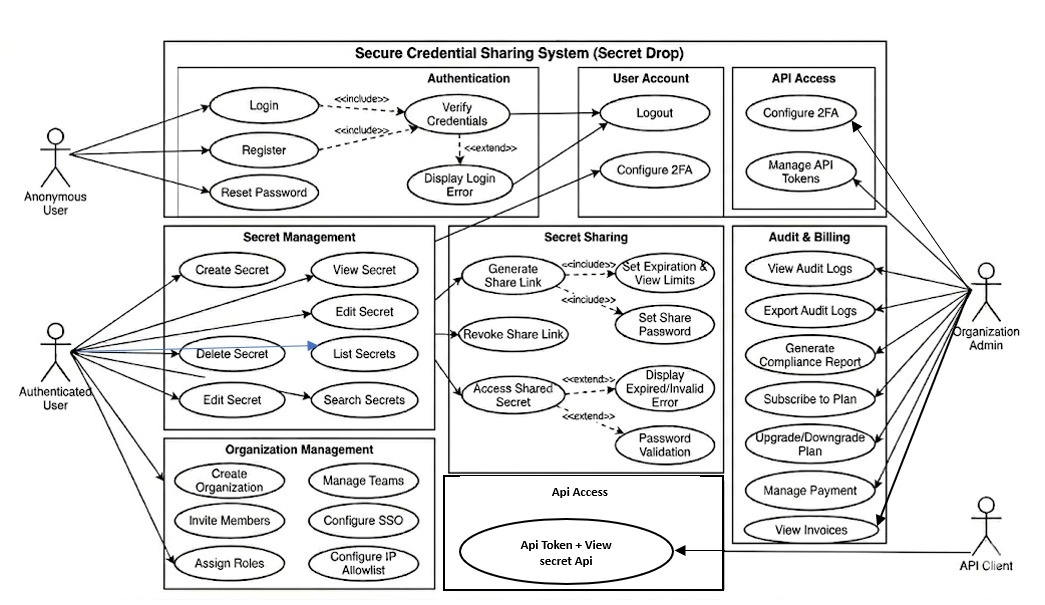
\includegraphics[width=\linewidth,height=0.88\textheight,keepaspectratio]{assets/Usecase Diagram.jpeg}
\end{center}
\blocksep
\textit{Explanation:} The use case diagram illustrates all system interactions across actors. Anonymous User can register, login, and reset password. Authenticated User creates, views, edits, deletes, lists, and searches secrets; generates and revokes share links; sets optional passwords on shares; manages API tokens; and configures 2FA. External Recipient accesses shared secrets via links without an account. Organization Admin creates organizations, invites members, assigns roles (Owner, Admin, Member), manages teams, configures SSO, and sets IP allowlist. API Client uses tokens for programmatic access to view and list secrets. Authenticated users view audit logs; admins export logs, generate compliance reports, subscribe to plans, upgrade/downgrade, manage payment methods, and view invoices.

\subsubsection{Use Case Description}
\addcontentsline{toc}{subsubsection}{Use Case Description}

\begin{table}[H]
  \centering
  \small
  \caption{UC-007: Create Secret}
  \begin{tabular}{@{}p{2.4cm}>{\raggedright\arraybackslash}p{10.2cm}@{}}
    \toprule
    \textbf{Field} & \textbf{Description}                                                                                                                                           \\
    \midrule
    Use Case ID    & UC-007                                                                                                                                                         \\
    \hline
    Name           & Create Secret                                                                                                                                                  \\
    \hline
    Actor          & Authenticated User                                                                                                                                             \\
    \hline
    Preconditions  & User logged in; belongs to organization; org under secret limit                                                                                                \\
    \hline
    Main Flow      & User enters name, content (max 1MB); selects encryption mode; sets expiration (1h--30d) and max views; optionally assigns to team; system encrypts and stores. \\
    \hline
    Postconditions & Secret stored; audit log created; appears in list.                                                                                                             \\
    \hline
    FR References  & FR-SCRT-1, 2, 3, 4, 5                                                                                                                                          \\
    \bottomrule
  \end{tabular}
\end{table}

\begin{table}[H]
  \centering
  \small
  \caption{UC-013: Generate Share Link}
  \begin{tabular}{@{}p{2.4cm}>{\raggedright\arraybackslash}p{10.2cm}@{}}
    \toprule
    \textbf{Field} & \textbf{Description}                                                                                                                       \\
    \midrule
    Use Case ID    & UC-013                                                                                                                                     \\
    \hline
    Name           & Generate Share Link                                                                                                                        \\
    \hline
    Actor          & Authenticated User (Secret Owner)                                                                                                          \\
    \hline
    Preconditions  & User logged in; has access to secret; secret not expired                                                                                   \\
    \hline
    Main Flow      & User clicks Share; configures expiration, max views, optional password; system generates 64-char token; saves share record; displays link. \\
    \hline
    Postconditions & Share link created; audit log entry; link ready for distribution.                                                                          \\
    \hline
    FR References  & FR-SHR-1, 2, 3, 4, 5                                                                                                                       \\
    \bottomrule
  \end{tabular}
\end{table}

\begin{table}[H]
  \centering
  \small
  \caption{UC-014: Access Shared Secret}
  \begin{tabular}{@{}p{2.4cm}>{\raggedright\arraybackslash}p{10.2cm}@{}}
    \toprule
    \textbf{Field} & \textbf{Description}                                                                                                                                                              \\
    \midrule
    Use Case ID    & UC-014                                                                                                                                                                            \\
    \hline
    Name           & Access Shared Secret                                                                                                                                                              \\
    \hline
    Actor          & Anonymous User / External Recipient                                                                                                                                               \\
    \hline
    Preconditions  & Valid share link; not expired; view count under max                                                                                                                               \\
    \hline
    Main Flow      & User opens link; system validates; prompts password if protected; displays secret; increments view count; logs access; deletes if burn-on-read; deactivates if max views reached. \\
    \hline
    Postconditions & Secret displayed; view count incremented; audit created.                                                                                                                          \\
    \hline
    FR References  & FR-SHR-5, 6, 7, 8                                                                                                                                                                 \\
    \bottomrule
  \end{tabular}
\end{table}

\subsubsection{Class Diagram}
\addcontentsline{toc}{subsubsection}{Class Diagram}

\begin{center}
  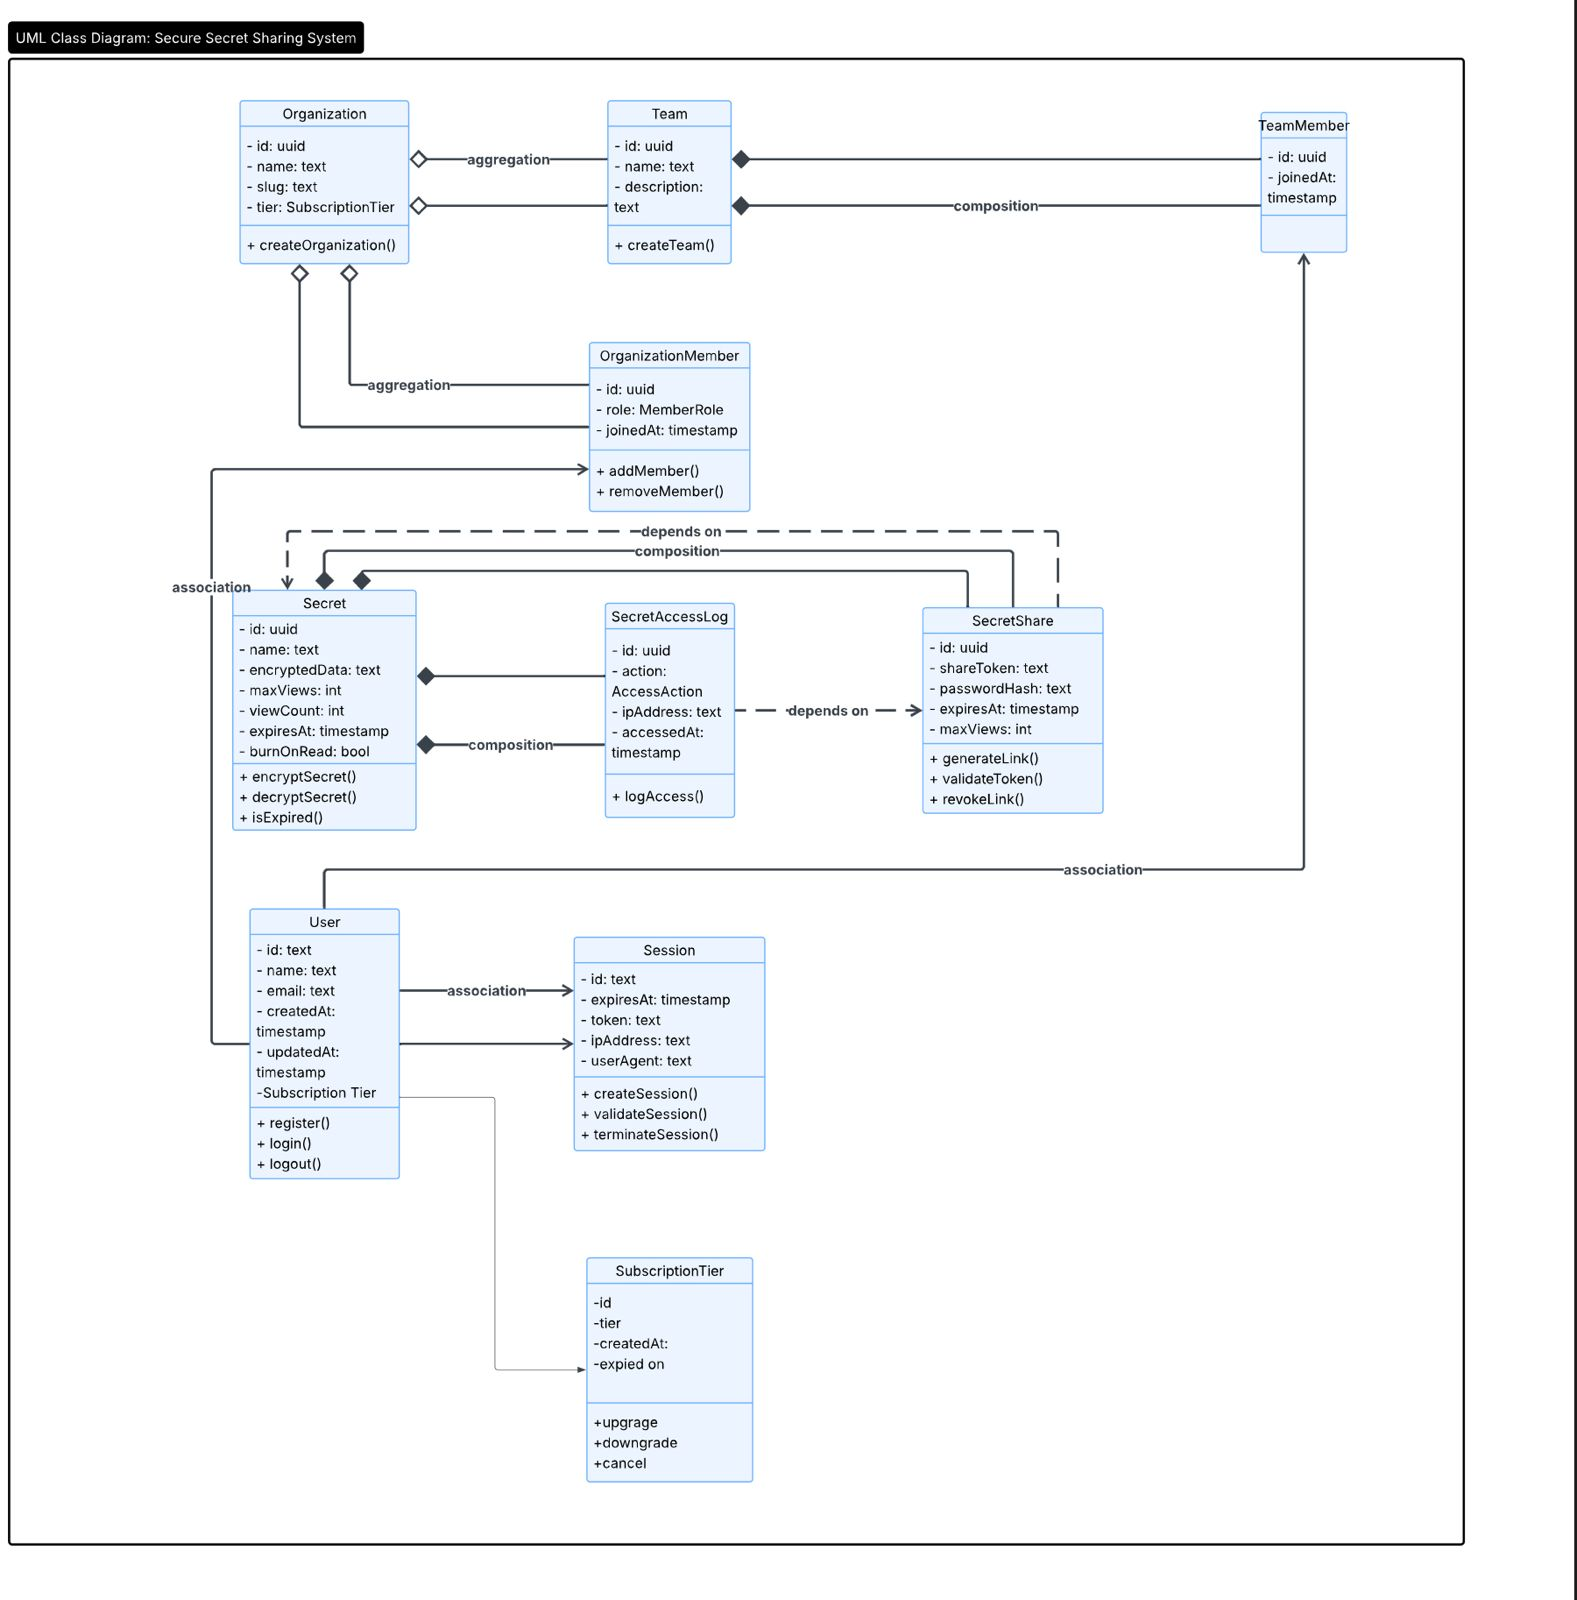
\includegraphics[width=\linewidth,height=0.88\textheight,keepaspectratio]{assets/class.jpeg}
\end{center}
\blocksep
\textit{Explanation:} The class diagram illustrates the complete domain model of Secret Drop. User holds identity (id, name, email) and has many Sessions. Organization aggregates OrganizationMembers (with role-based access) and Teams. Secret stores encrypted data with expiration, view limits, and burn-on-read settings. SecretShare holds share tokens and optional password protection. SecretAccessLog records all access for audit compliance.

\subsubsection{Sequence Diagram}
\addcontentsline{toc}{subsubsection}{Sequence Diagram}

The sequence diagram illustrates the key interactions for creating secrets, generating share links, and accessing shared secrets.

\begin{center}
  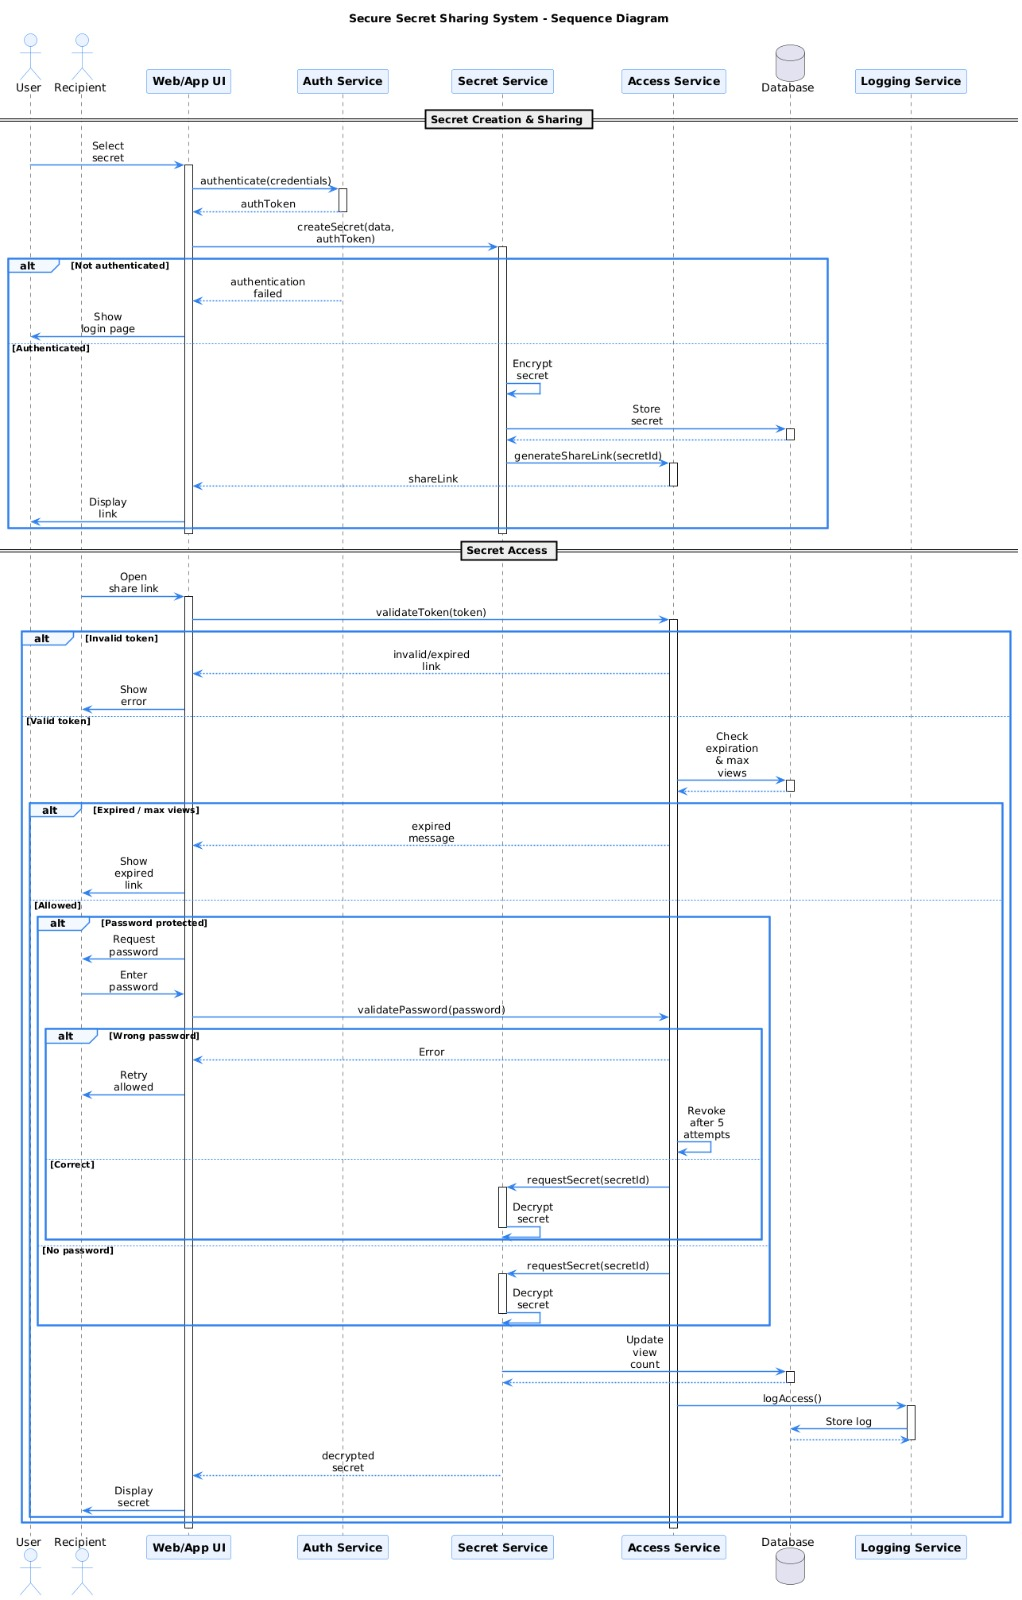
\includegraphics[width=\linewidth,height=0.88\textheight,keepaspectratio]{assets/Sequence Diagram.jpeg}
\end{center}
\blocksep
\textit{Explanation:} The sequence diagram shows three main flows. (1) Create Secret: User opens form; UI validates session; user submits; API checks limit, encrypts content, stores in DB, logs to audit; success returned to user. (2) Generate Share Link: User clicks Share; API fetches secret, generates 64-char token, stores SecretShare, logs event; share URL returned for copying. (3) Access Shared Secret: Recipient opens link; API validates token, expiration, view count; if password protected, prompts and validates; fetches and decrypts secret; increments view count; logs access; displays content. Invalid or expired links show error.

\subsubsection{Activity Diagram}
\addcontentsline{toc}{subsubsection}{Activity Diagram}

The activity diagram illustrates the workflows for share link creation and recipient access.

\begin{center}
  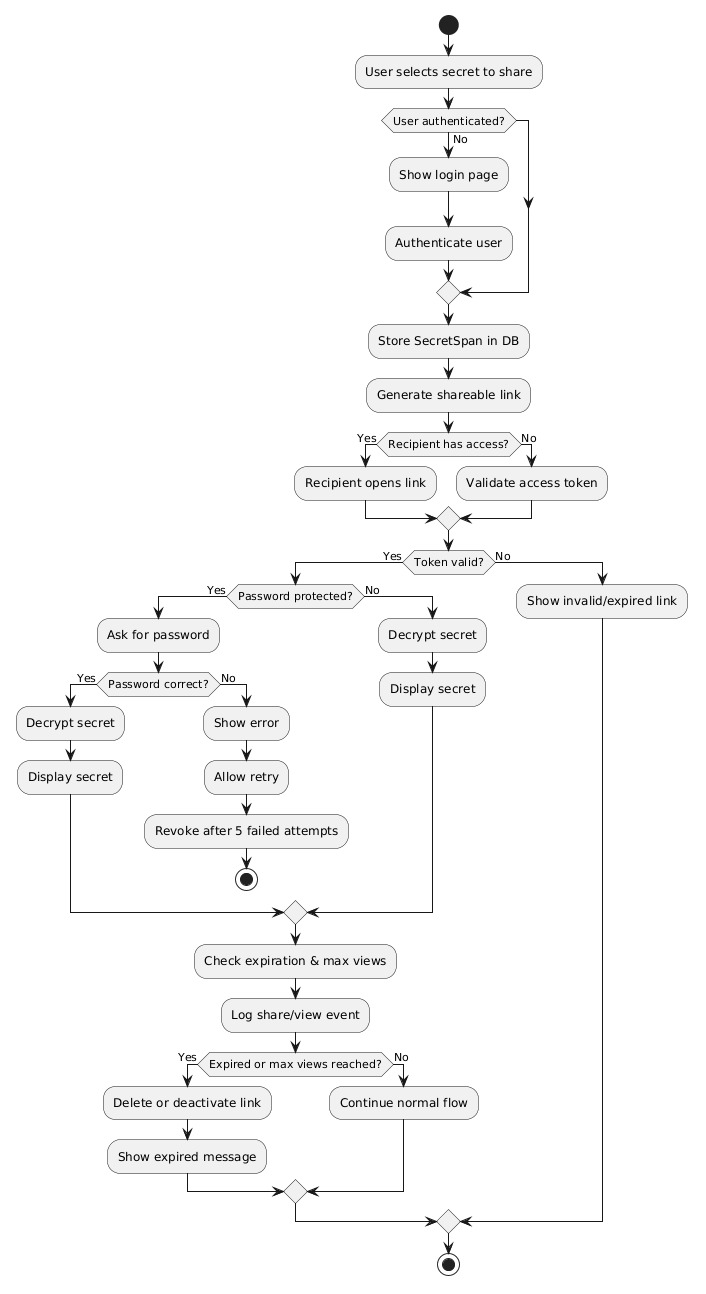
\includegraphics[width=\linewidth,height=0.88\textheight,keepaspectratio]{assets/Activity Diagram.jpeg}
\end{center}
\blocksep
\textit{Explanation:} The activity diagram covers two main workflows. (1) Share Link Creation: User selects secret; system checks authentication (redirect to login if needed); verifies permission; user configures expiration, max views, optional password; system generates token, stores share, logs event; link ready. (2) Recipient Access: Recipient opens link; system validates token; checks expiration and max views; if password protected, prompts (5 failed attempts revokes link); decrypts and displays secret; increments view count; if burn-on-read or max views reached, deletes or deactivates.

% ==================== 5. Testing ====================
\section{Testing}

\subsection{End-to-End (E2E) Test Suite}

The project uses Playwright for end-to-end testing. All E2E test specifications reside in the \texttt{e2e/} directory. The following tables list functional test cases (input--action--assertion) for the four main modules. Tests that verify only static UI rendering are excluded.

% --- 5.1 Authentication ---
\subsubsection{Authentication}
\addcontentsline{toc}{subsubsection}{Authentication}

{\footnotesize
\begin{longtable}{@{}p{1.4cm}p{2.6cm}p{3.3cm}p{3.8cm}p{1.4cm}p{0.8cm}@{}}
  \toprule
  \textbf{TC ID} & \textbf{Description} & \textbf{Input} & \textbf{Expected Result} & \textbf{Actual} & \textbf{Status} \\
  \midrule
  \endfirsthead
  \toprule
  \textbf{TC ID} & \textbf{Description} & \textbf{Input} & \textbf{Expected Result} & \textbf{Actual} & \textbf{Status} \\
  \midrule
  \endhead
  \hline
  \multicolumn{6}{r}{\textit{Continued on next page}} \\
  \endfoot
  \bottomrule
  \endlastfoot

  TC-AUTH-01 &
  Login fails with empty fields &
  Click sign-in without entering credentials &
  Form validation prevents submission; stays on login page &
  As expected &
  Pass \\
  \hline

  TC-AUTH-02 &
  Login fails with invalid credentials &
  Enter wrong email and password; click sign-in &
  Shows ``User not found'' or ``Invalid password'' error &
  As expected &
  Pass \\
  \hline

  TC-AUTH-03 &
  Successful login redirects to dashboard &
  Enter valid test user email and password; click sign-in &
  Redirects to \texttt{/dashboard} &
  As expected &
  Pass \\
  \hline

  TC-AUTH-04 &
  Signup rejects short password &
  Enter name, email, password ``short'' (7 chars); click create &
  Validation prevents submission &
  As expected &
  Pass \\
  \hline

  TC-AUTH-05 &
  Signup requires terms acceptance &
  Fill valid data; skip terms checkbox; click create &
  Form prevents submission without terms acceptance &
  As expected &
  Pass \\
  \hline

  TC-AUTH-06 &
  Successful signup redirects to dashboard &
  Fill unique email, name, valid password ($\geq$8 chars); accept terms; submit &
  Redirects to \texttt{/dashboard} &
  As expected &
  Pass \\
\end{longtable}
}

% --- 5.2 Secret Management ---
\subsubsection{Secret Management}
\addcontentsline{toc}{subsubsection}{Secret Management}

{\footnotesize
\begin{longtable}{@{}p{1.4cm}p{2.6cm}p{3.3cm}p{3.8cm}p{1.4cm}p{0.8cm}@{}}
  \toprule
  \textbf{TC ID} & \textbf{Description} & \textbf{Input} & \textbf{Expected Result} & \textbf{Actual} & \textbf{Status} \\
  \midrule
  \endfirsthead
  \toprule
  \textbf{TC ID} & \textbf{Description} & \textbf{Input} & \textbf{Expected Result} & \textbf{Actual} & \textbf{Status} \\
  \midrule
  \endhead
  \hline
  \multicolumn{6}{r}{\textit{Continued on next page}} \\
  \endfoot
  \bottomrule
  \endlastfoot

  TC-SCRT-01 &
  Search filters secrets by name &
  Type ``nonexistent-xyz'' in search field on secrets list &
  Results filtered; no matching secret shown &
  As expected &
  Pass \\
  \hline

  TC-SCRT-02 &
  Free tier restricts expiration options &
  Open expiration selector on free tier account &
  Shows 1\,h, 1\,d, 7\,d; hides 30\,d and Never &
  As expected &
  Pass \\
  \hline

  TC-SCRT-03 &
  Burn-on-read disabled on free tier &
  View burn-on-read toggle on free tier account &
  Toggle disabled with ``Pro/Business only'' label &
  As expected &
  Pass \\
  \hline

  TC-SCRT-04 &
  Create form rejects empty submission &
  Click create without filling name or value &
  Shows validation errors for required fields &
  As expected &
  Pass \\
  \hline

  TC-SCRT-05 &
  Secret creation with valid inputs &
  Fill name, value, password ($\geq$8 chars); select 1\,h expiration; submit &
  Secret created; redirects to detail page &
  As expected &
  Pass \\
  \hline

  TC-SCRT-06 &
  Decrypt with correct password &
  Enter correct password; click ``View Secret'' &
  Decrypted content displayed &
  As expected &
  Pass \\
  \hline

  TC-SCRT-07 &
  Decrypt fails with wrong password &
  Enter incorrect password; click ``View Secret'' &
  Shows ``Failed to decrypt'' error &
  As expected &
  Pass \\
  \hline

  TC-SCRT-08 &
  Delete requires confirmation &
  Click delete on secret detail page &
  Confirmation dialog appears before deletion &
  As expected &
  Pass \\
  \hline

  TC-SCRT-09 &
  Public decrypt without login &
  Navigate to share link while logged out; enter password; click Decrypt &
  Secret decrypted without requiring login &
  As expected &
  Pass \\
  \hline

  TC-SCRT-10 &
  Invalid share link shows error &
  Navigate to invalid share link; enter password; click Decrypt &
  Shows ``Failed'' or ``Not found'' error &
  As expected &
  Pass \\
\end{longtable}
}

% --- 5.3 Dashboard ---
\subsubsection{Dashboard}
\addcontentsline{toc}{subsubsection}{Dashboard}

{\footnotesize
\begin{longtable}{@{}p{1.4cm}p{2.6cm}p{3.3cm}p{3.8cm}p{1.4cm}p{0.8cm}@{}}
  \toprule
  \textbf{TC ID} & \textbf{Description} & \textbf{Input} & \textbf{Expected Result} & \textbf{Actual} & \textbf{Status} \\
  \midrule
  \endfirsthead
  \toprule
  \textbf{TC ID} & \textbf{Description} & \textbf{Input} & \textbf{Expected Result} & \textbf{Actual} & \textbf{Status} \\
  \midrule
  \endhead
  \hline
  \multicolumn{6}{r}{\textit{Continued on next page}} \\
  \endfoot
  \bottomrule
  \endlastfoot

  TC-DASH-01 &
  Unauthenticated access blocked &
  Clear cookies; navigate to \texttt{/dashboard} &
  Redirects to landing page; shows sign-in link &
  As expected &
  Pass \\
\end{longtable}
}

% --- 5.4 Settings ---
\subsubsection{Settings}
\addcontentsline{toc}{subsubsection}{Settings}

{\footnotesize
\begin{longtable}{@{}p{1.4cm}p{2.6cm}p{3.3cm}p{3.8cm}p{1.4cm}p{0.8cm}@{}}
  \toprule
  \textbf{TC ID} & \textbf{Description} & \textbf{Input} & \textbf{Expected Result} & \textbf{Actual} & \textbf{Status} \\
  \midrule
  \endfirsthead
  \toprule
  \textbf{TC ID} & \textbf{Description} & \textbf{Input} & \textbf{Expected Result} & \textbf{Actual} & \textbf{Status} \\
  \midrule
  \endhead
  \hline
  \multicolumn{6}{r}{\textit{Continued on next page}} \\
  \endfoot
  \bottomrule
  \endlastfoot

  TC-SETT-01 &
  Update profile display name &
  Change name; click ``Save Changes'' &
  Shows success toast ``Profile updated'' &
  As expected &
  Pass \\
  \hline

  TC-SETT-02 &
  Billing period toggle changes prices &
  Toggle from monthly to yearly on billing page &
  Prices update; ``Save 20\%'' label appears &
  As expected &
  Pass \\
  \hline

  TC-SETT-03 &
  Create and revoke API token &
  Create token with name; then click revoke &
  Token appears in list; removed after revocation &
  As expected &
  Pass \\
\end{longtable}
}

\subsection{Test Coverage Summary}

\begin{table}[H]
  \centering
  \small
  \caption{E2E Test Coverage by Main Module}
  \begin{tabular}{@{}lccp{5.5cm}@{}}
    \toprule
    \textbf{Module} & \textbf{Test Cases} & \textbf{Test Files} & \textbf{Key Flows Covered} \\
    \midrule
    Authentication    & 6 & 2 & Login (valid/invalid/empty), signup (validation, terms, success) \\
    \hline
    Secret Management & 10 & 4 & CRUD, search, encrypt/decrypt, tier gating, public sharing \\
    \hline
    Dashboard         & 1 & 1 & Auth guard redirect \\
    \hline
    Settings          & 3 & 3 & Profile update, billing toggle, API token lifecycle \\
    \hline
    \textbf{Total}    & \textbf{20} & \textbf{10} & \\
    \bottomrule
  \end{tabular}
\end{table}

% ==================== 6. Git Version Control ====================
\section{Git Version Control}

\subsection{Repository Commit History}

Version control was used throughout development to keep the project traceable and collaborative. The commit history shows iterative progress with focused updates for features, fixes, refactoring, testing, and deployment configuration. This made it easier to review work incrementally and identify when specific changes were introduced.

\begin{figure}[H]
  \centering
  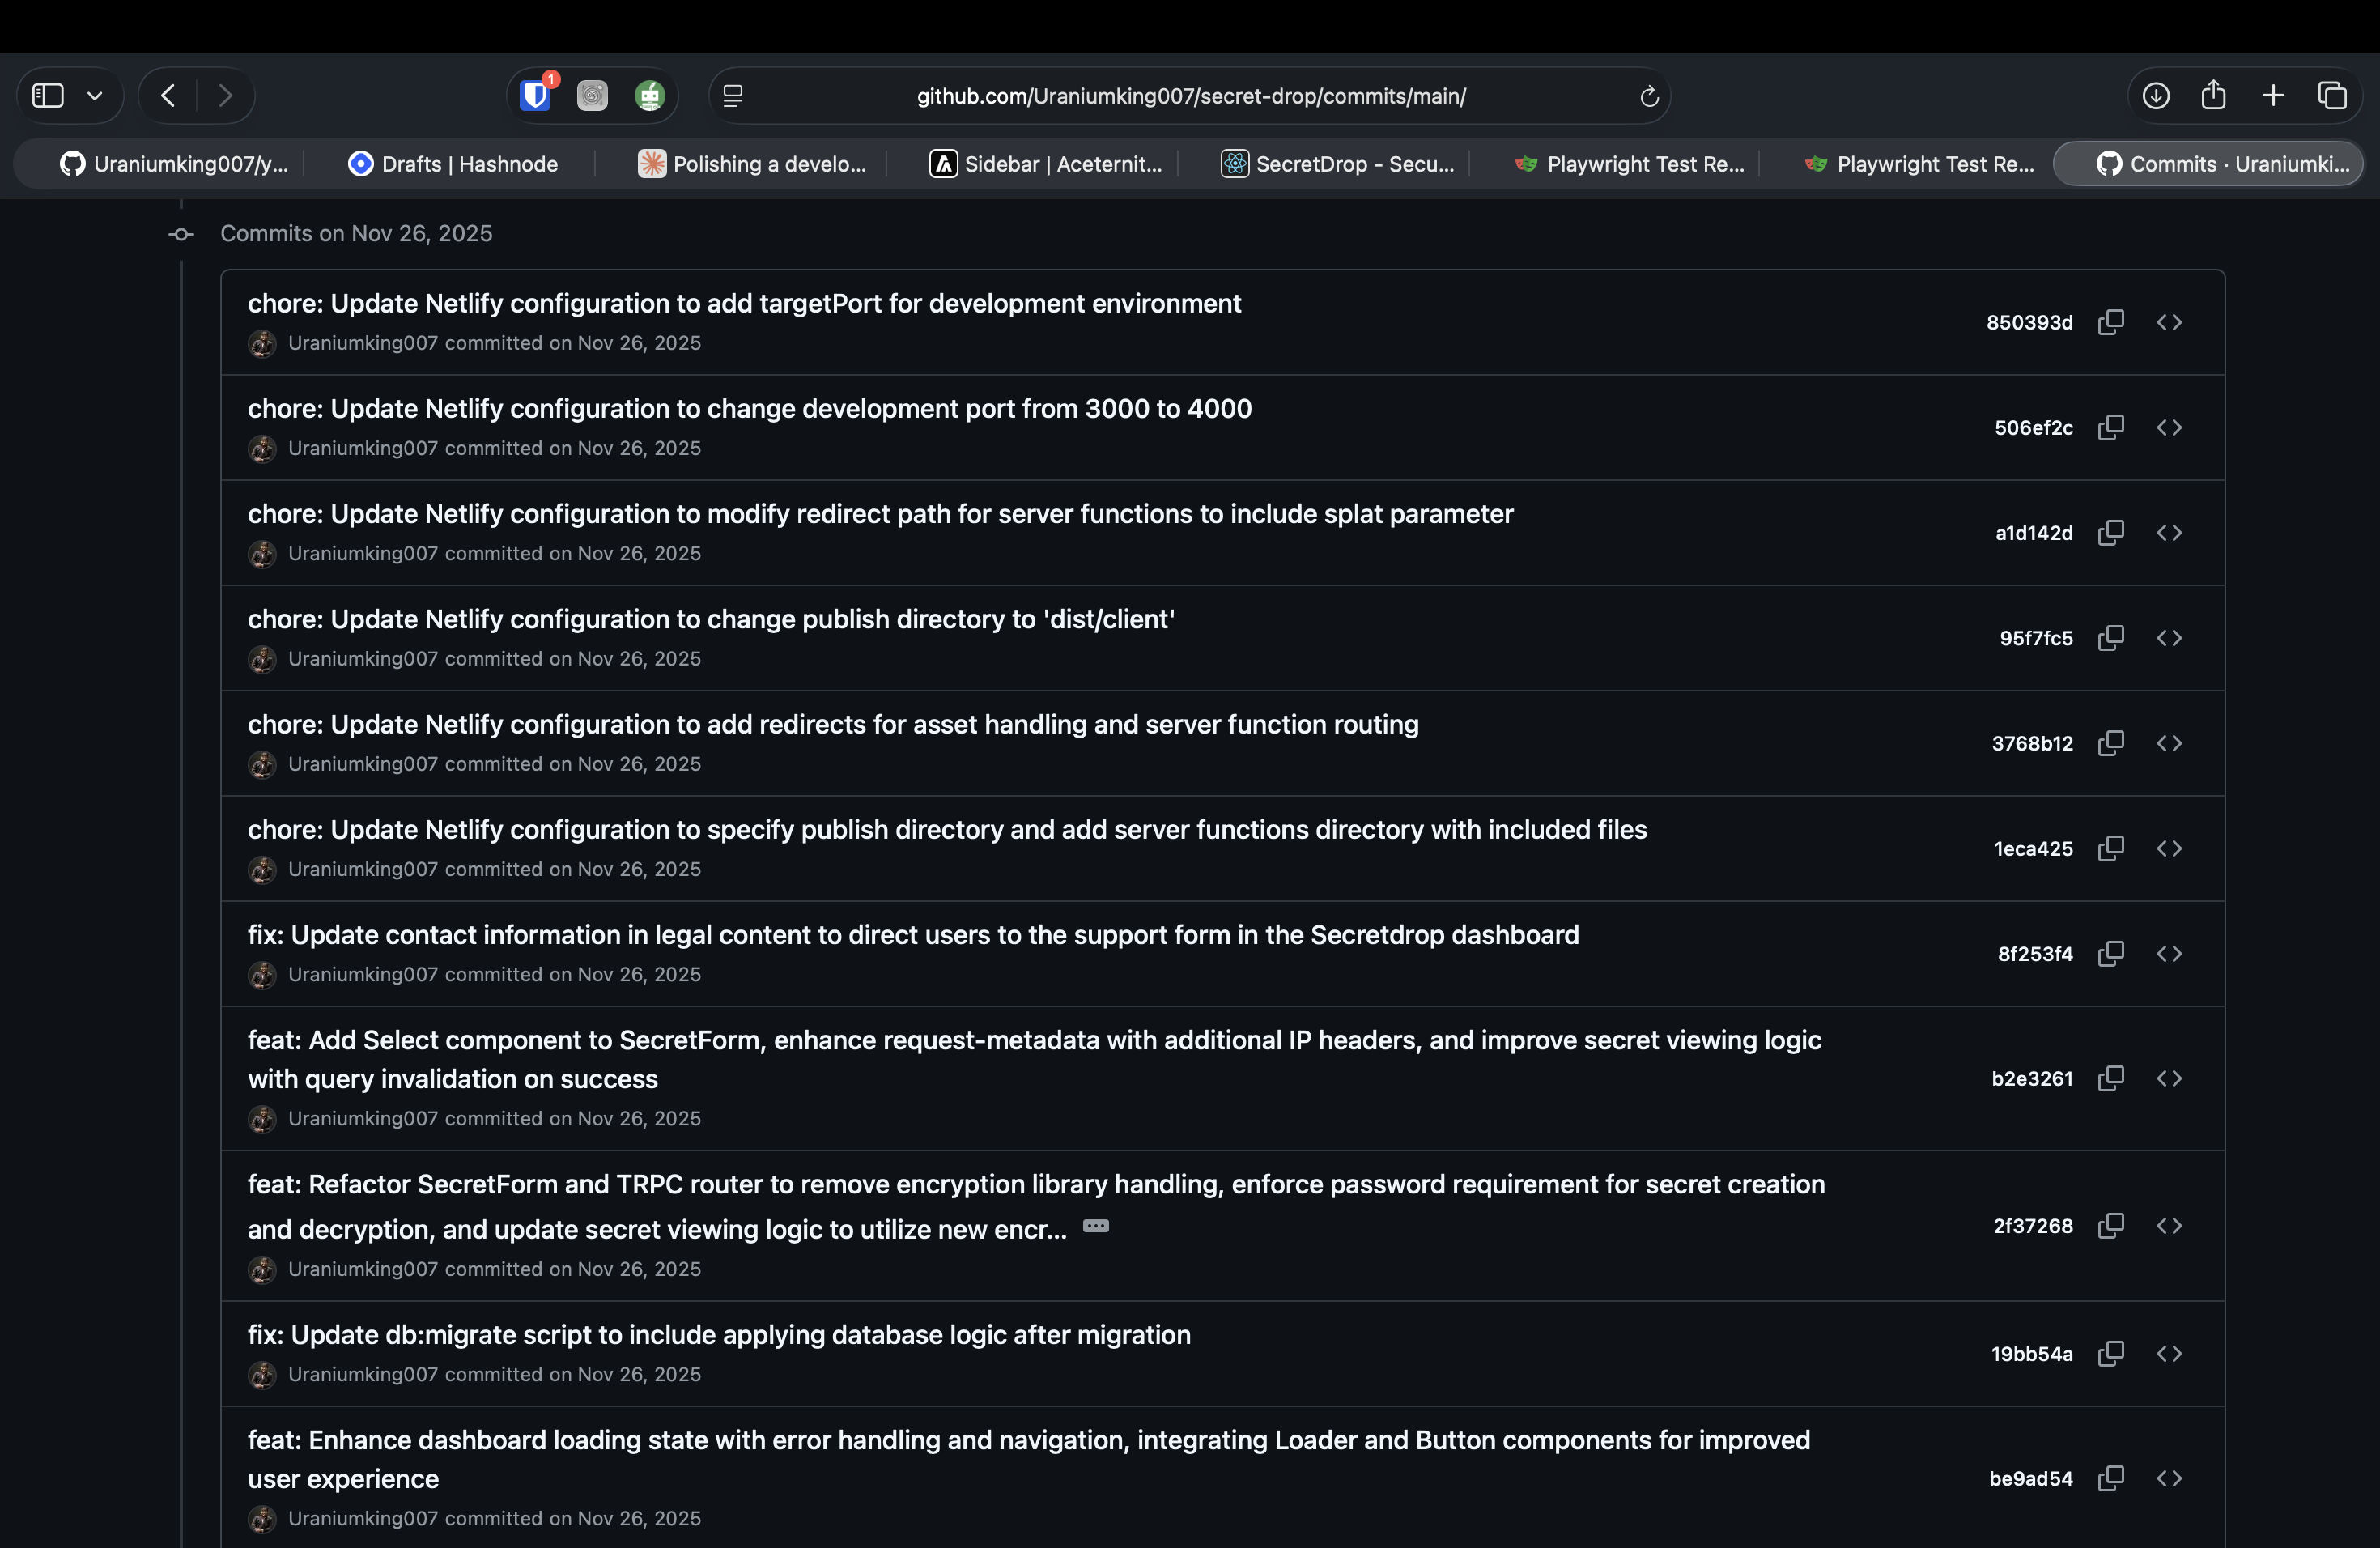
\includegraphics[width=\linewidth,keepaspectratio]{assets/github1.png}
  \caption{Main branch commit history showing feature, fix, and configuration updates}
\end{figure}

\begin{figure}[H]
  \centering
  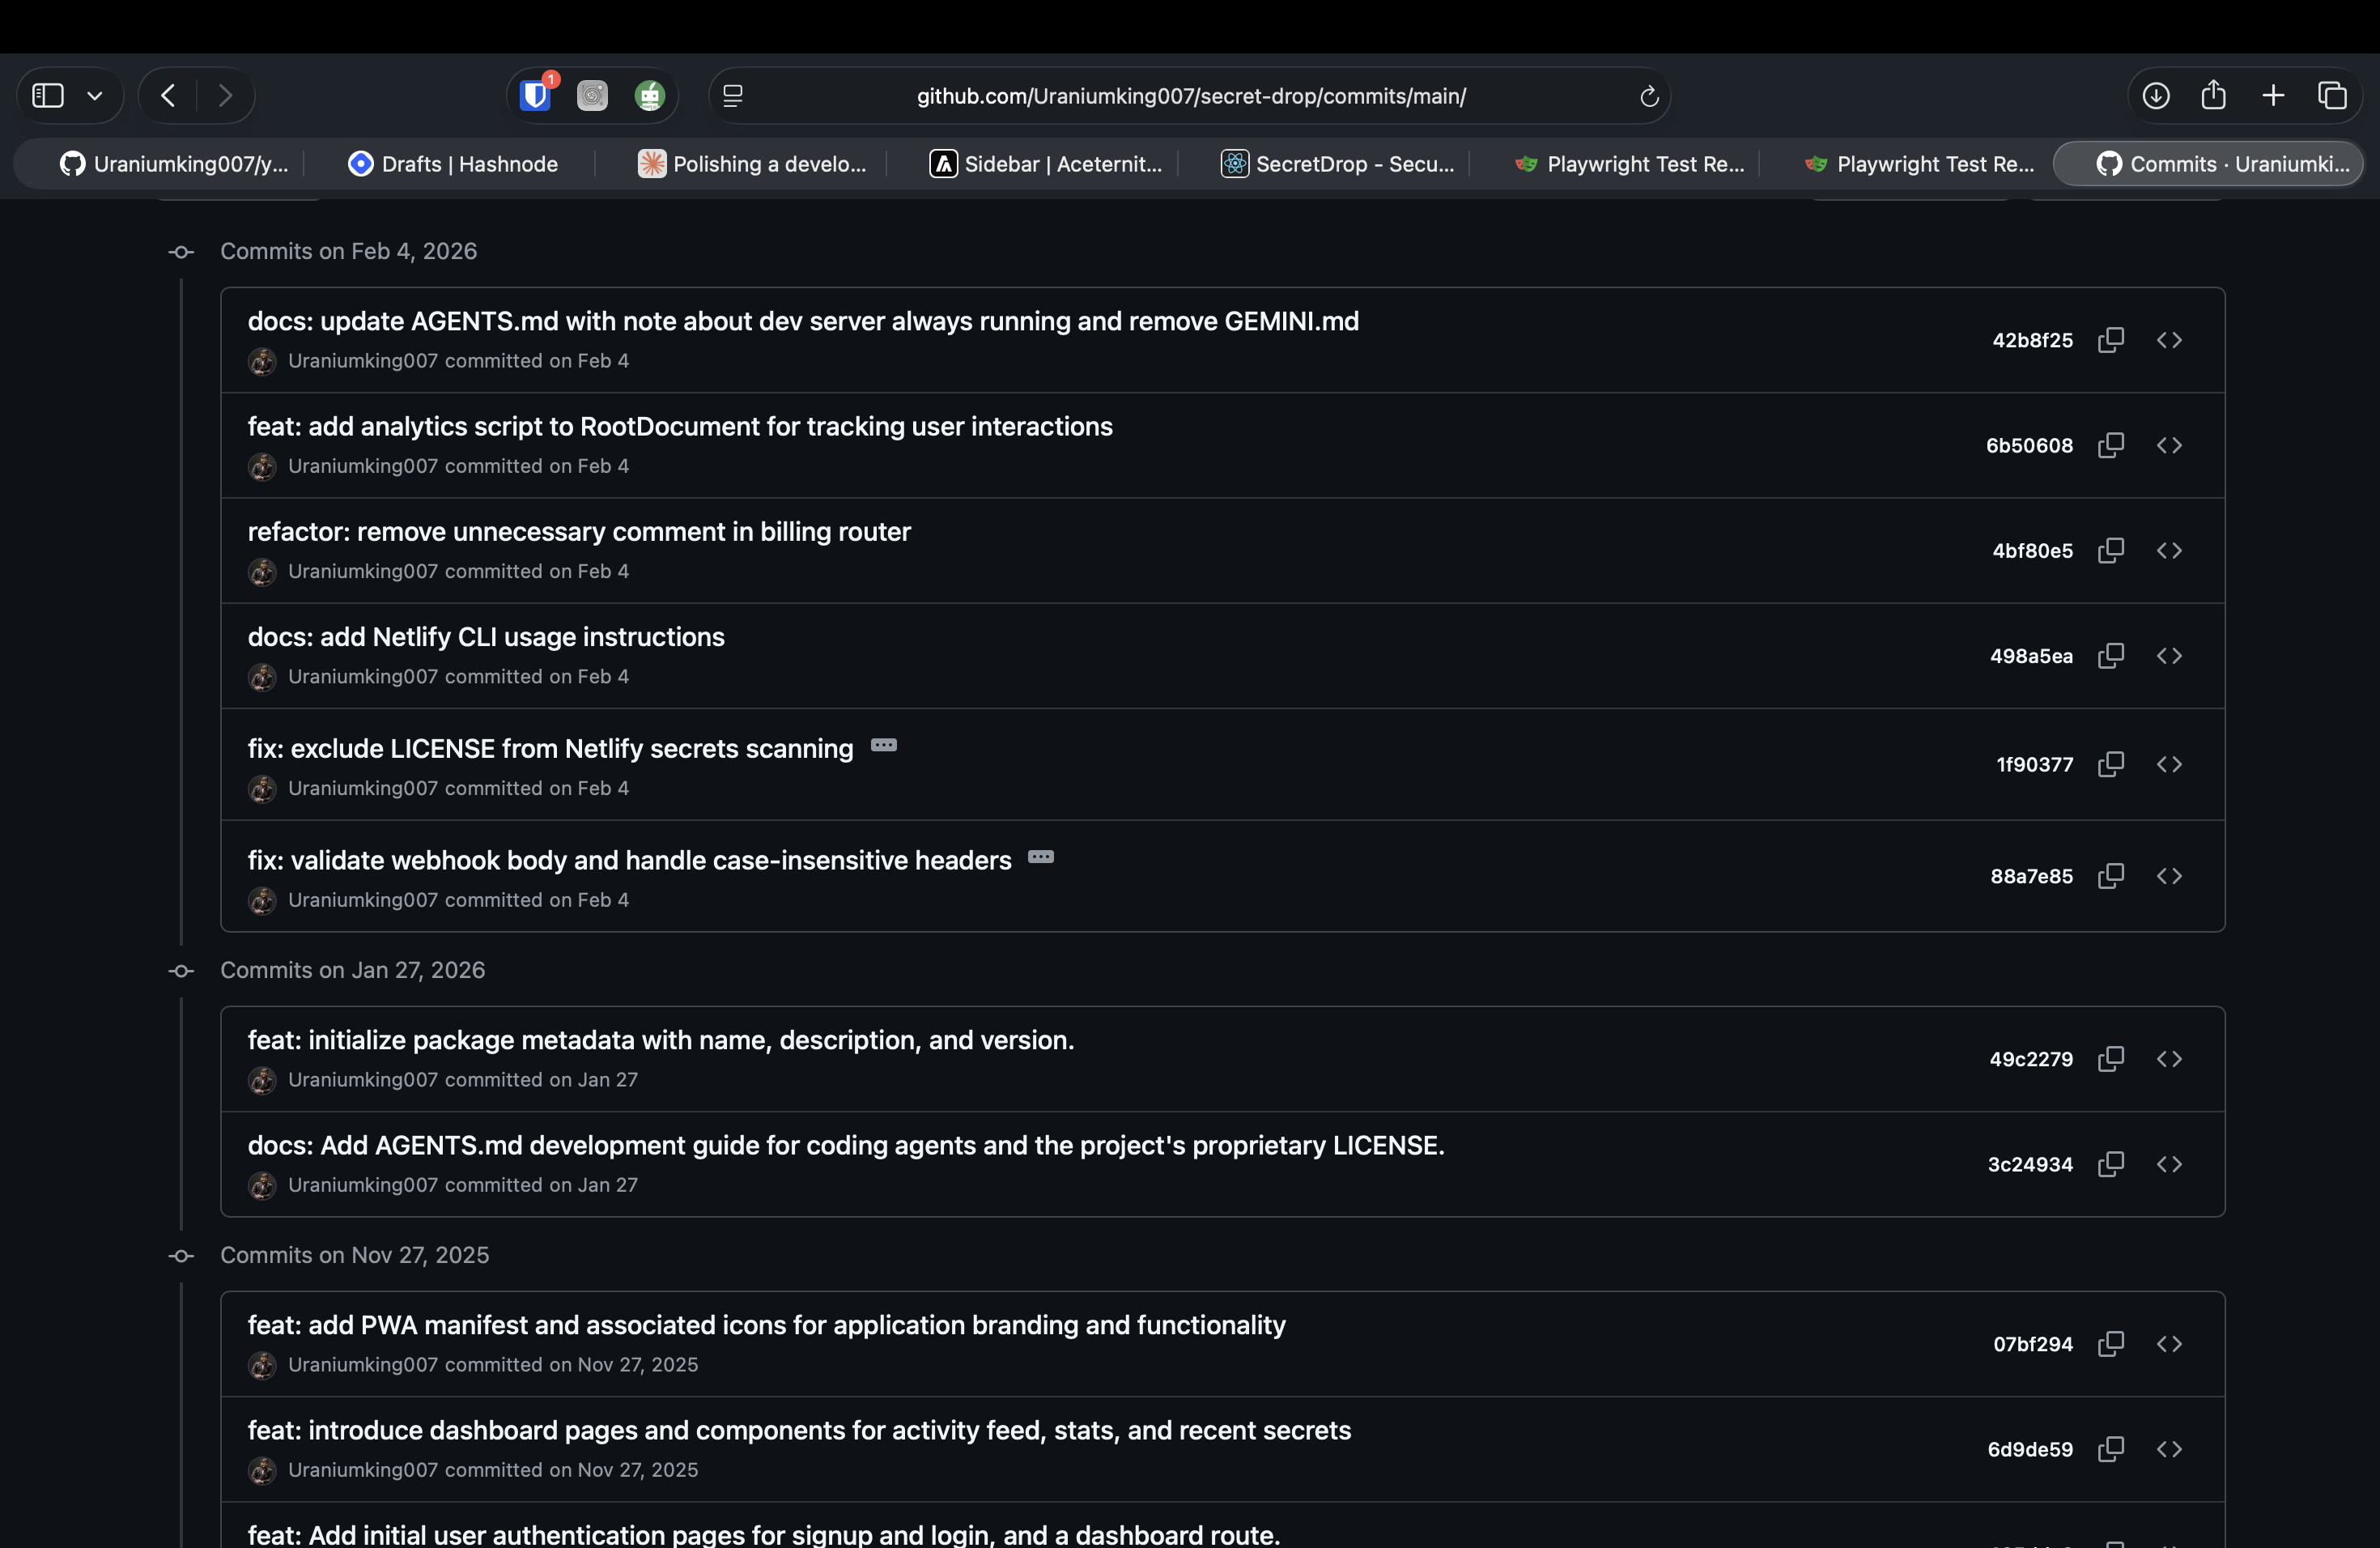
\includegraphics[width=\linewidth,keepaspectratio]{assets/github2.png}
  \caption{Recent commits highlighting documentation, analytics, and deployment improvements}
\end{figure}

\subsection{Collaboration and Repository Structure}

The project repository structure demonstrates organized collaboration between team members. Work is separated into clear directories (application code, migrations, tests, scripts, and docs), allowing parallel development without conflicts. Frequent commits from multiple contributors indicate active coordination and continuous integration of changes.

\begin{figure}[H]
  \centering
  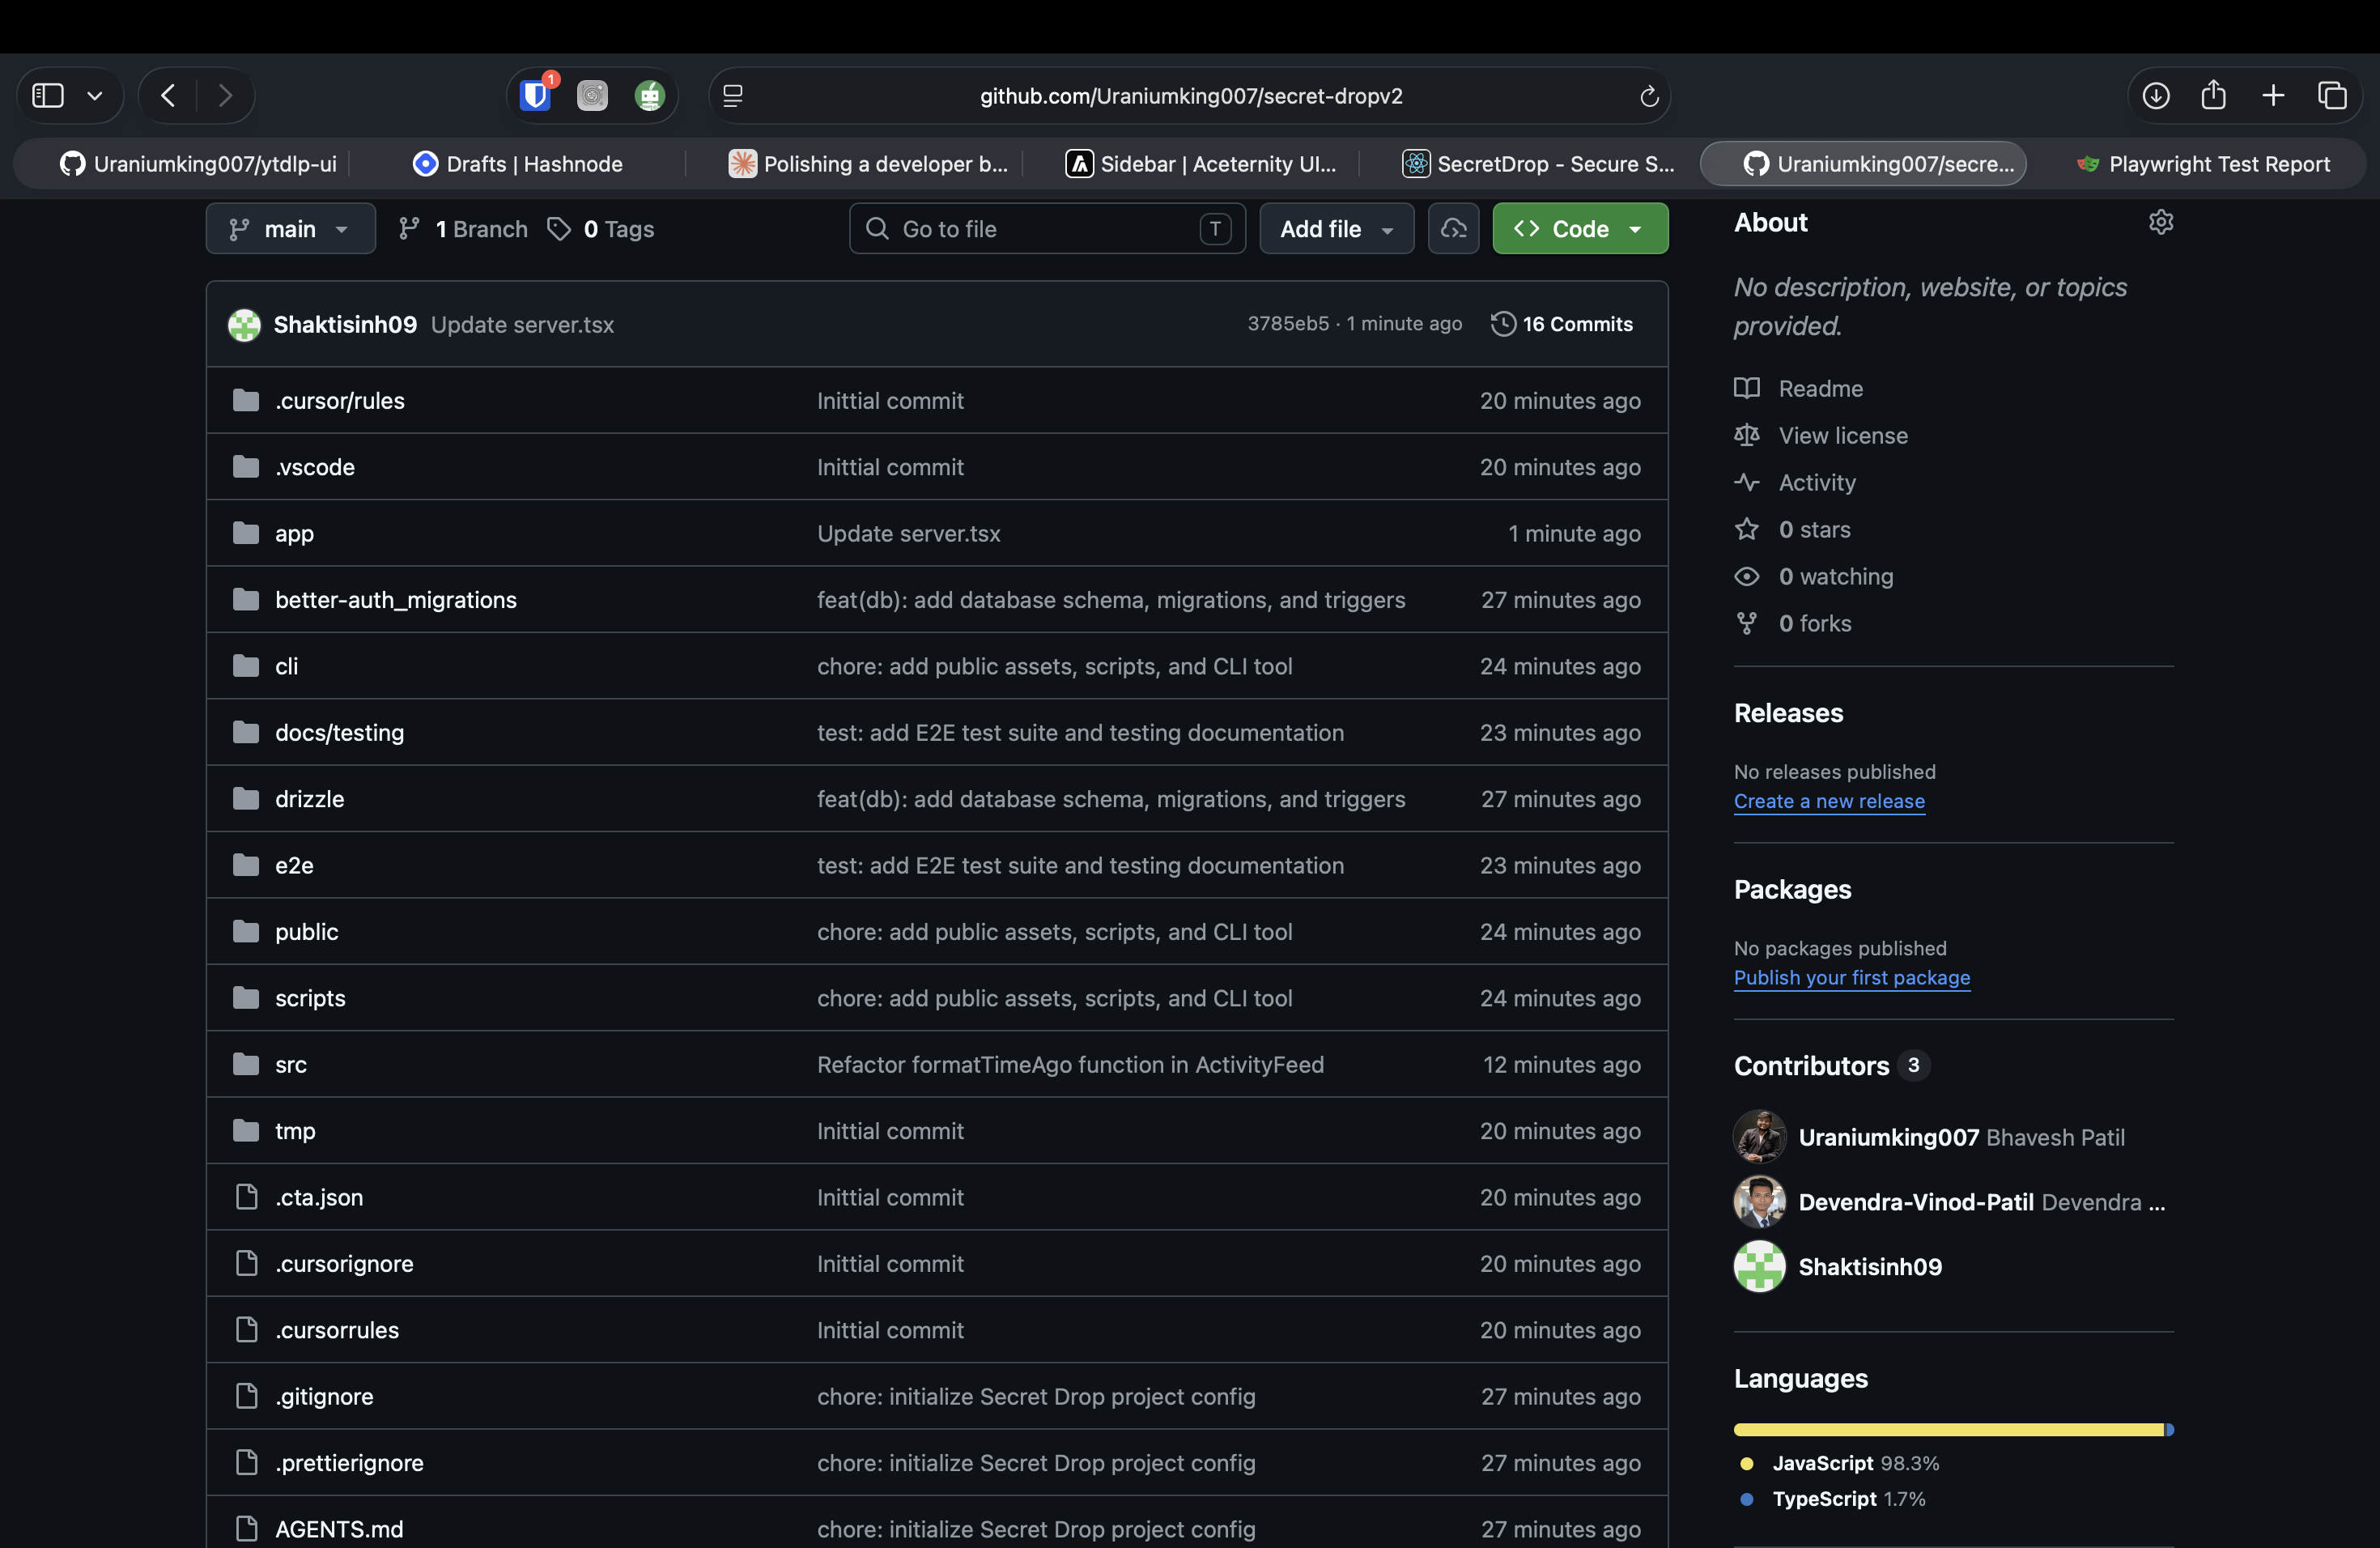
\includegraphics[width=\linewidth,keepaspectratio]{assets/collab.png}
  \caption{Repository overview showing team collaboration and modular project structure}
\end{figure}

% ==================== 7. References ====================
\section{References}

\subsection{Technical Documentation}
\begin{itemize}[leftmargin=*]
  \item TanStack: \url{https://tanstack.com/}
  \item React 19: \url{https://react.dev/}
  \item Drizzle ORM: \url{https://orm.drizzle.team/}
  \item Better Auth: \url{https://www.better-auth.com/}
  \item tRPC: \url{https://trpc.io/}
  \item Tailwind CSS: \url{https://tailwindcss.com/}
\end{itemize}

\subsection{Security \& Compliance}
\begin{itemize}[leftmargin=*]
  \item OWASP Top 10: \url{https://owasp.org/www-project-top-ten/}
  \item NIST Crypto Standards: \url{https://csrc.nist.gov/}
  \item Web Crypto API: \url{https://developer.mozilla.org/docs/Web/API/Web_Crypto_API}
  \item GDPR: \url{https://gdpr.eu/}
  \item PCI-DSS: \url{https://www.pcisecuritystandards.org/}
  \item Stripe: \url{https://stripe.com/docs}
\end{itemize}

\subsection{Standards}
\begin{itemize}[leftmargin=*]
  \item Agile Manifesto: \url{https://agilemanifesto.org/}
  \item Scrum Guide: \url{https://scrumguides.org/}
  \item UML: \url{https://www.uml.org/}
  \item REST API: \url{https://restfulapi.net/}
  \item OpenAPI: \url{https://spec.openapis.org/}
\end{itemize}

% ==================== Appendix A: Glossary ====================
\appendix
\section*{Appendix A: Glossary}

\begin{table}[H]
  \centering
  \small
  \begin{tabular}{@{}p{3.5cm}p{10cm}@{}}
    \toprule
    \textbf{Term}          & \textbf{Definition}                                            \\
    \midrule
    AES-256-GCM            & Advanced Encryption Standard, 256-bit key, Galois/Counter Mode \\
    \hline
    Burn-on-Read           & Secret auto-deletes after first view                           \\
    \hline
    CIDR                   & Classless Inter-Domain Routing for IP ranges                   \\
    \hline
    Client-Side Encryption & Encryption on user device before sending to server             \\
    \hline
    JAMstack               & JavaScript, APIs, Markup architecture                          \\
    \hline
    OAuth 2.0              & Open standard for authorization                                \\
    \hline
    OIDC                   & OpenID Connect, auth layer on OAuth 2.0                        \\
    \hline
    PBKDF2                 & Password-Based Key Derivation Function 2                       \\
    \hline
    RBAC                   & Role-Based Access Control                                      \\
    \hline
    SAML                   & Security Assertion Markup Language for SSO                     \\
    \hline
    SSO                    & Single Sign-On                                                 \\
    \hline
    tRPC                   & TypeScript RPC framework                                       \\
    \hline
    TOTP                   & Time-based One-Time Password                                   \\
    \bottomrule
  \end{tabular}
\end{table}

\section*{Appendix B: Acronyms}

\begin{minipage}{\linewidth}
  \small\raggedright
  API (Application Programming Interface), AES (Advanced Encryption Standard), CI/CD (Continuous Integration/Deployment), CCPA (California Consumer Privacy Act), CSP (Content Security Policy), CSRF (Cross-Site Request Forgery), GDPR (General Data Protection Regulation), HSTS (HTTP Strict Transport Security), IV (Initialization Vector), OAuth (Open Authorization), PBKDF2 (Password-Based Key Derivation Function 2), PCI-DSS (Payment Card Industry Data Security Standard), RBAC (Role-Based Access Control), SAML (Security Assertion Markup Language), SDLC (Software Development Life Cycle), SSO (Single Sign-On), TLS (Transport Layer Security), TOTP (Time-based One-Time Password), UML (Unified Modeling Language), WCAG (Web Content Accessibility Guidelines).
\end{minipage}

\end{document}
